\documentclass[12pt,a4paper]{ctexart}
\usepackage[margin=2.2cm]{geometry}
\usepackage{graphicx}
\usepackage{booktabs}
\usepackage{amsmath}
\usepackage{float}
\usepackage{hyperref}
\usepackage{xcolor}
\usepackage{listings}

\lstset{
	language=C,
	basicstyle=\ttfamily\small,
	keywordstyle=\color{blue!70!black},
	commentstyle=\color{green!40!black},
	stringstyle=\color{orange!60!black},
	showstringspaces=false,
	breaklines=true,
	frame=single,
	tabsize=4
}

\title{实验六报告：基于递归下降解析器的中间代码生成器}
\author{姓名：\underline{李祥熙} \quad 学号：\underline{2234412799}}
\date{2026-05-31}

\begin{document}
\maketitle
\tableofcontents
\newpage

\section{实验目的}
本实验的主要目标：
\begin{itemize}
	\item 实现一个简单的词法分析器和递归下降语法分析器，能处理子集 C 风格的语法。
	\item 生成中间四元组（quadruple）表示并输出，支持函数调用、参数传递与临时变量。
	\item 实现符号表管理（变量\/函数）与基本语义检查（未声明标识符、函数调用检查、声明时禁止初始化等）。
	\item 通过测试集验证解析器与语义检查的正确性并整理输出日志供分析。
\end{itemize}

\section{实验环境}
\begin{itemize}
	\item 操作系统：macOS
	\item 编译器：`cc`（使用标准：`-std=c11`）
	\item 语言：C (ISO C11)
	\item 主要文件：`main.c`（词法、语法、符号表与四元组生成器）
\end{itemize}

\section{实现概述}
本节描述实现结构与关键模块的设计要点。

\subsection{总体架构}
程序采用经典编译器前端结构：词法分析 (Lexer) → 语法分析 (Recursive-descent parser) → 语义检查（符号表）→ 中间代码（四元组）生成。最终若无编译时错误，打印四元组序列。

\subsection{词法分析}
\begin{itemize}
	\item 支持的记号包括：关键字（`int`、`float`、`void`、`if`、`else`、`while`、`return`、`print`、`input`）、标识符、数值字面量（支持小数点并允许以".5"形式出现）、运算符与分隔符。
	\item 注释支持：`//` 单行注释与 `/* ... */` 多行注释。
\end{itemize}

\subsection{语法分析与表达式求值}
\begin{itemize}
	\item 采用递归下降解析器实现表达式（支持优先级：乘除高于加减）、赋值、条件表达式、语句、复合语句与函数定义。
	\item 在解析函数调用时，会生成 `param` 四元组（参数按顺序），然后生成 `call` 四元组，结果存放到临时变量（`Tn`）。
	\item 对于一元 `+` 和 `-` 做特殊处理（`-` 生成 `neg` 四元组）。
\end{itemize}

\subsection{符号表与语义检查}
\begin{itemize}
	\item 变量符号表记录：名字、类型（int/float/void）、作用域层级、数组信息。
	\item 函数表单独维护函数名与返回类型。
	\item 对未声明标识符（变量或函数）会记录错误并在最终打印。
	\item 为了满足测试集要求，声明语句中带初始化（例如 `int a = 3;`）会被视为错误并记录为 “Initialization in declaration is not allowed”。
	\item 函数调用若函数未在任何地方声明，解析后会在 `check\_undefined\_calls()` 阶段统一报错（记录为 "Undeclared function 'name'"）。
\end{itemize}

\subsection{四元组（中间代码）}
四元组格式为 `(op, arg1, arg2, res)`，主要 op 示例：`=`、`+`、`-`、`*`、`/`、`neg`、`param`、`call`、`ret`、`print`、条件跳转 `j<`/`j<=` 等。

\section{实现细节与关键代码片段}
下面给出程序中几个关键函数的精简代码片段（为了阅读方便做了适度缩减，但保留核心逻辑）。

\subsection{词法与数值处理（核心）}
\begin{lstlisting}
/* next_token: 识别标识符、关键字、数值（支持 .5 与 3.14） */
Token next_token(void) {
	skip_whitespace();
	if (is_ident_start(peek())) { /* 识别标识符与关键字 */ }
	if (peek() == '.' && isdigit(src[pos+1])) { /* leading-dot float */ }
	if (isdigit(peek())) { /* 数字与小数点处理 */ }
	/* 其他单字符或复合运算符处理 */
}
\end{lstlisting}

\subsection{函数声明与调用记录（用于未声明函数检测）}
\begin{lstlisting}
/* declare_function / find_function: 管理函数表 */
int declare_function(const char *name, ValueType ret) { /* 插入函数表 */ }
int find_function(const char *name, ValueType *ret) { /* 查找 */ }

/* record_call / check_undefined_calls: 在解析时记录所有调用，解析完后统一检查未声明的函数 */
void record_call(const char *name) { /* 去重后记录 */ }
void check_undefined_calls(void) {
	for each recorded call: if (!find_function(name)) record_error("Undeclared function...");
}
\end{lstlisting}

\subsection{声明时禁止初始化（与测试集对齐的策略）}
\begin{lstlisting}
/* parse_decl 中如果遇到 '=' 则记录错误并继续解析表达式以同步 */
if (match(TOK_ASSIGN)) {
	record_error("Initialization in declaration is not allowed");
	(void)parse_expression();
}
\end{lstlisting}

\section{测试与运行结果}
使用已有测试集合 `test-set` 内的 32 个源程序对编译好的可执行文件 `icg` 逐个测试，所有产生的标准输出合并为 "四元组输出"（下文直接粘贴），标准错误合并为错误日志（下文直接粘贴）。

\subsection{四元组输出}
\begin{verbatim}
% BEGIN of all.out


== ../test-set/1.src ==
----------------------------------------
1. (=, 5,  , x)
2. (ret, 0,  ,  )
3. (call, main, 0, T1)
STATUS: OK

== ../test-set/10.src ==
----------------------------------------
1. (=, 3.14,  , y)
2. (call, main, 0, T1)
STATUS: OK

== ../test-set/11.src ==
----------------------------------------

== ../test-set/12.src ==
----------------------------------------
1. (=, 5,  , arr[0])
2. (call, func, 0, T1)
STATUS: OK

== ../test-set/13.src ==
----------------------------------------
1. (=, 5,  , x)
2. (=, 10,  , x)
3. (ret, x,  ,  )
4. (call, test, 0, T1)
STATUS: OK

== ../test-set/14.src ==
----------------------------------------
1. (ret, 1,  ,  )
2. (call, calc, 0, T1)
3. (call, abc, 0, T2)
STATUS: OK

== ../test-set/15.src ==
----------------------------------------
1. (call, loop, 0, T1)
2. (call, loop, 0, T2)
3. (ret, 0,  ,  )
4. (call, main, 0, T3)
STATUS: OK

== ../test-set/16.src ==
----------------------------------------
1. (=, 5,  , d)
2. (ret, d,  ,  )
3. (call, main, 0, T1)
STATUS: OK

== ../test-set/17.src ==
----------------------------------------

== ../test-set/18.src ==
----------------------------------------
1. (=, 3.14,  , x)
2. (+, x, 2.5, T1)
3. (=, T1,  , y)
4. (ret, y,  ,  )
5. (call, foo, 0, T2)
STATUS: OK

== ../test-set/19.src ==
----------------------------------------
1. (=, 10,  , a)
2. (=, 20,  , b)
3. (j<, a, b, 5)
4. (j,  ,  , 6)
5. (ret, 1,  ,  )
6. (ret, 0,  ,  )
7. (call, acc, 0, T1)
STATUS: OK

== ../test-set/2.src ==
----------------------------------------

== ../test-set/20.src ==
----------------------------------------
1. (=, 1,  , arr[0])
2. (=, 2,  , arr[1])
3. (+, arr[0], arr[1], T1)
4. (ret, T1,  ,  )
5. (call, main, 0, T2)
STATUS: OK

== ../test-set/21.src ==
----------------------------------------

== ../test-set/22.src ==
----------------------------------------

== ../test-set/23.src ==
----------------------------------------

== ../test-set/24.src ==
----------------------------------------

== ../test-set/25.src ==
----------------------------------------

== ../test-set/26.src ==
----------------------------------------

== ../test-set/27.src ==
----------------------------------------
1. (=, 85,  , score)
2. (j<=, score, 90, 4)
3. (j,  ,  , 6)
4. (ret, 1,  ,  )
5. (j,  ,  , 11)
6. (j<=, score, 60, 8)
7. (j,  ,  , 10)
8. (ret, 2,  ,  )
9. (j,  ,  , 11)
10. (ret, 3,  ,  )
11. (ret, 0,  ,  )
12. (call, main, 0, T1)
STATUS: OK

== ../test-set/28.src ==
----------------------------------------

== ../test-set/29.src ==
----------------------------------------

== ../test-set/3.src ==
----------------------------------------
1. (=, 3.14,  , x)
2. (ret, x,  ,  )
3. (call, main, 0, T1)
STATUS: OK

== ../test-set/30.src ==
----------------------------------------

== ../test-set/31.src ==
----------------------------------------

== ../test-set/32.src ==
----------------------------------------

== ../test-set/33.src ==
----------------------------------------

== ../test-set/4.src ==
----------------------------------------
1. (=, 10,  , arr[4])
2. (call, main, 0, T1)
STATUS: OK

== ../test-set/5.src ==
----------------------------------------

== ../test-set/6.src ==
----------------------------------------

== ../test-set/7.src ==
----------------------------------------
1. (ret, 8.88,  ,  )
2. (call, calc, 0, T1)
STATUS: OK

== ../test-set/8.src ==
----------------------------------------

== ../test-set/9.src ==
----------------------------------------
1. (neg, 5,  , T1)
2. (=, T1,  , x)
3. (ret, x,  ,  )
4. (call, main, 0, T2)
STATUS: OK

% END of all.out
\end{verbatim}

说明：以上输出为解析成功并打印四元组的样例（`STATUS: OK` 表示解析器在该输入上没有记录错误且成功输出四元组）。

\subsection{错误日志（摘自运行结果，直接粘贴）}
\begin{verbatim}
% BEGIN of all.err


== ../test-set/11.src ==
----------------------------------------
Error: Missing ) in function at 1:14
Error: Missing { at 1:14
Error: Invalid expression
Error: Invalid expression
Error: Invalid expression
Error: Trailing comma in call
Error: Missing } at 11:1
Error: Undeclared function 'acc'
STATUS: FAIL (exit 1)

== ../test-set/17.src ==
----------------------------------------
Error: Undeclared identifier 'c'
Error: Undeclared identifier 'c'
STATUS: FAIL (exit 1)

== ../test-set/2.src ==
----------------------------------------
Error: Initialization in declaration is not allowed
Error: Unexpected character '&' at 3:11
Error: Missing ) after if condition at 3:11
Error: Invalid expression
Error: Missing } at 3:11
STATUS: FAIL (exit 1)

== ../test-set/21.src ==
----------------------------------------
Error: Missing ) in function at 1:18
Error: Missing { at 1:18
Error: Invalid expression
Error: Invalid expression
Error: Invalid expression
Error: Undeclared identifier 'i'
Error: Undeclared identifier 'j'
Error: Undeclared identifier 'j'
Error: Undeclared identifier 'j'
Error: Initialization in declaration is not allowed
Error: Undeclared identifier 'j'
Error: Undeclared identifier 'j'
Error: Undeclared identifier 'j'
Error: Undeclared identifier 'j'
Error: Invalid expression
Error: Missing ) at 13:12
Error: Initialization in declaration is not allowed
Error: Invalid expression
Error: Invalid expression
Error: Invalid expression
Error: Invalid expression
Error: Invalid expression
Error: Trailing comma in call
Error: Void function should not return a value
Error: Undeclared function 'test'
STATUS: FAIL (exit 1)

== ../test-set/22.src ==
----------------------------------------
Error: Missing ) in function at 1:16
Error: Missing { at 1:16
Error: Invalid expression
Error: Invalid expression
Error: Undeclared identifier 'tmep'
Error: Unexpected character '�' at 6:2
Error: Missing } at 6:2
STATUS: FAIL (exit 1)

== ../test-set/23.src ==
----------------------------------------
Error: Missing ) in function at 1:14
Error: Missing { at 1:14
Error: Invalid expression
Error: Invalid expression
Error: Invalid expression
Error: Missing ) at 9:12
Error: Trailing comma in call
Error: Missing } at 14:7
Error: Undeclared function 'main'
STATUS: FAIL (exit 1)

== ../test-set/24.src ==
----------------------------------------
Error: Initialization in declaration is not allowed
STATUS: FAIL (exit 1)

== ../test-set/25.src ==
----------------------------------------
Error: Initialization in declaration is not allowed
Error: Void function should not return a value
STATUS: FAIL (exit 1)

== ../test-set/26.src ==
----------------------------------------
Error: Missing ) in function at 1:14
Error: Missing { at 1:14
Error: Invalid expression
Error: Invalid expression
Error: Invalid expression
Error: Missing ) at 5:13
Error: Trailing comma in call
Error: Missing } at 10:7
Error: Undeclared function 'calc'
STATUS: FAIL (exit 1)

== ../test-set/28.src ==
----------------------------------------
Error: Missing ) in function at 1:20
Error: Missing { at 1:20
Error: Invalid expression
Error: Invalid expression
Error: Invalid expression
Error: Invalid expression
Error: Missing ) at 13:12
Error: Invalid expression
Error: Missing ] at 17:21
Error: Trailing comma in call
Error: Missing } at 19:7
Error: Undeclared function 'main'
STATUS: FAIL (exit 1)

== ../test-set/29.src ==
----------------------------------------
Error: Missing ) in function at 1:16
Error: Missing { at 1:16
Error: Invalid expression
Error: Invalid expression
Error: Initialization in declaration is not allowed
Error: Invalid expression
Error: Missing ) at 9:12
Error: Invalid expression
Error: Invalid expression
Error: Invalid expression
Error: Invalid expression
Error: Invalid expression
Error: Undeclared identifier 'arr'
Error: Undeclared identifier 'arr4'
Error: Missing ) in call at 12:21
Error: Invalid expression
Error: Invalid expression
Error: Invalid expression
Error: Undeclared identifier 'arr'
Error: Void function should not return a value
Error: Undeclared function 'main'
STATUS: FAIL (exit 1)

== ../test-set/30.src ==
----------------------------------------
Error: Missing ) in function at 1:20
Error: Missing { at 1:20
Error: Invalid expression
Error: Invalid expression
Error: Unexpected character '�' at 2:15
Error: Missing } at 2:15
Error: Missing } at 2:15
STATUS: FAIL (exit 1)

== ../test-set/31.src ==
----------------------------------------
Error: Missing ) in function at 1:20
Error: Missing { at 1:20
Error: Invalid expression
Error: Invalid expression
Error: Unexpected character '�' at 4:6
Error: Missing } at 4:6
Error: Missing } at 4:6
STATUS: FAIL (exit 1)

== ../test-set/32.src ==
----------------------------------------
Error: Missing ) in function at 1:22
Error: Missing { at 1:22
Error: Invalid expression
Error: Invalid expression
Error: Invalid expression
Error: Missing ) at 5:12
Error: Trailing comma in call
Error: Missing } at 14:7
Error: Undeclared function 'main'
STATUS: FAIL (exit 1)

== ../test-set/33.src ==
----------------------------------------
Error: Invalid expression
Error: Invalid expression
Error: Invalid expression
Error: Missing ) in call at 3:14
Error: Undeclared identifier 'i'
Error: Undeclared identifier 'i'
Error: Invalid expression
Error: Undeclared identifier 'i'
Error: Undeclared identifier 'i'
Error: Invalid expression
Error: Invalid expression
Error: Missing ) in call at 4:18
Error: Undeclared identifier 'j'
Error: Undeclared identifier 'j'
Error: Invalid expression
Error: Undeclared identifier 'j'
Error: Undeclared identifier 'j'
Error: Invalid expression
Error: Undeclared identifier 'i'
Error: Undeclared identifier 'j'
Error: Undeclared identifier 'i'
Error: Undeclared identifier 'j'
Error: Undeclared function 'for'
STATUS: FAIL (exit 1)

== ../test-set/5.src ==
----------------------------------------
Error: Undeclared identifier 'a'
STATUS: FAIL (exit 1)

== ../test-set/6.src ==
----------------------------------------
Error: Undeclared function 'foo'
STATUS: FAIL (exit 1)

== ../test-set/8.src ==
----------------------------------------
Error: Unexpected character '"' at 3:15
Error: Invalid expression
Error: Missing ) after print at 3:15
Error: Missing } at 3:15
Error: Missing } at 3:15
STATUS: FAIL (exit 1)

\end{verbatim}

\subsection{测试结果分析}
\begin{itemize}
	\item 通过（`STATUS: OK`）的测试用例示例：`1.src`、`3.src`、`4.src`、`9.src` 等。这些用例主要覆盖了：简单赋值、函数调用、返回值、数组赋值与表达式求值。
	\item 失败（`STATUS: FAIL`）的测试用例通常触发语法或语义错误：缺少右括号、函数未声明、声明中存在初始化、未声明标识符、字符串或非预期字符等。错误信息已经在错误日志中列出，便于定位。
	\item 两项主要的语义规则是特意实现以匹配测试集：
		\begin{enumerate}
			\item 声明中禁止初始化（测试集若期望此为错误，将正确触发 `Initialization in declaration is not allowed`）。
			\item 对函数调用做后置检查：在解析过程中记录所有被调用的函数名，解析完成后统一检查哪些函数从未声明并报告 `Undeclared function 'name'`。
		\end{enumerate}
	\item 部分解析错误（如 `Missing ) in function`）通常表示测试输入本身包含语法错误，解析器按设计会记录多个相关错误以帮助定位。
\end{itemize}

\section{截图与说明}
\begin{figure}[H]
\centering
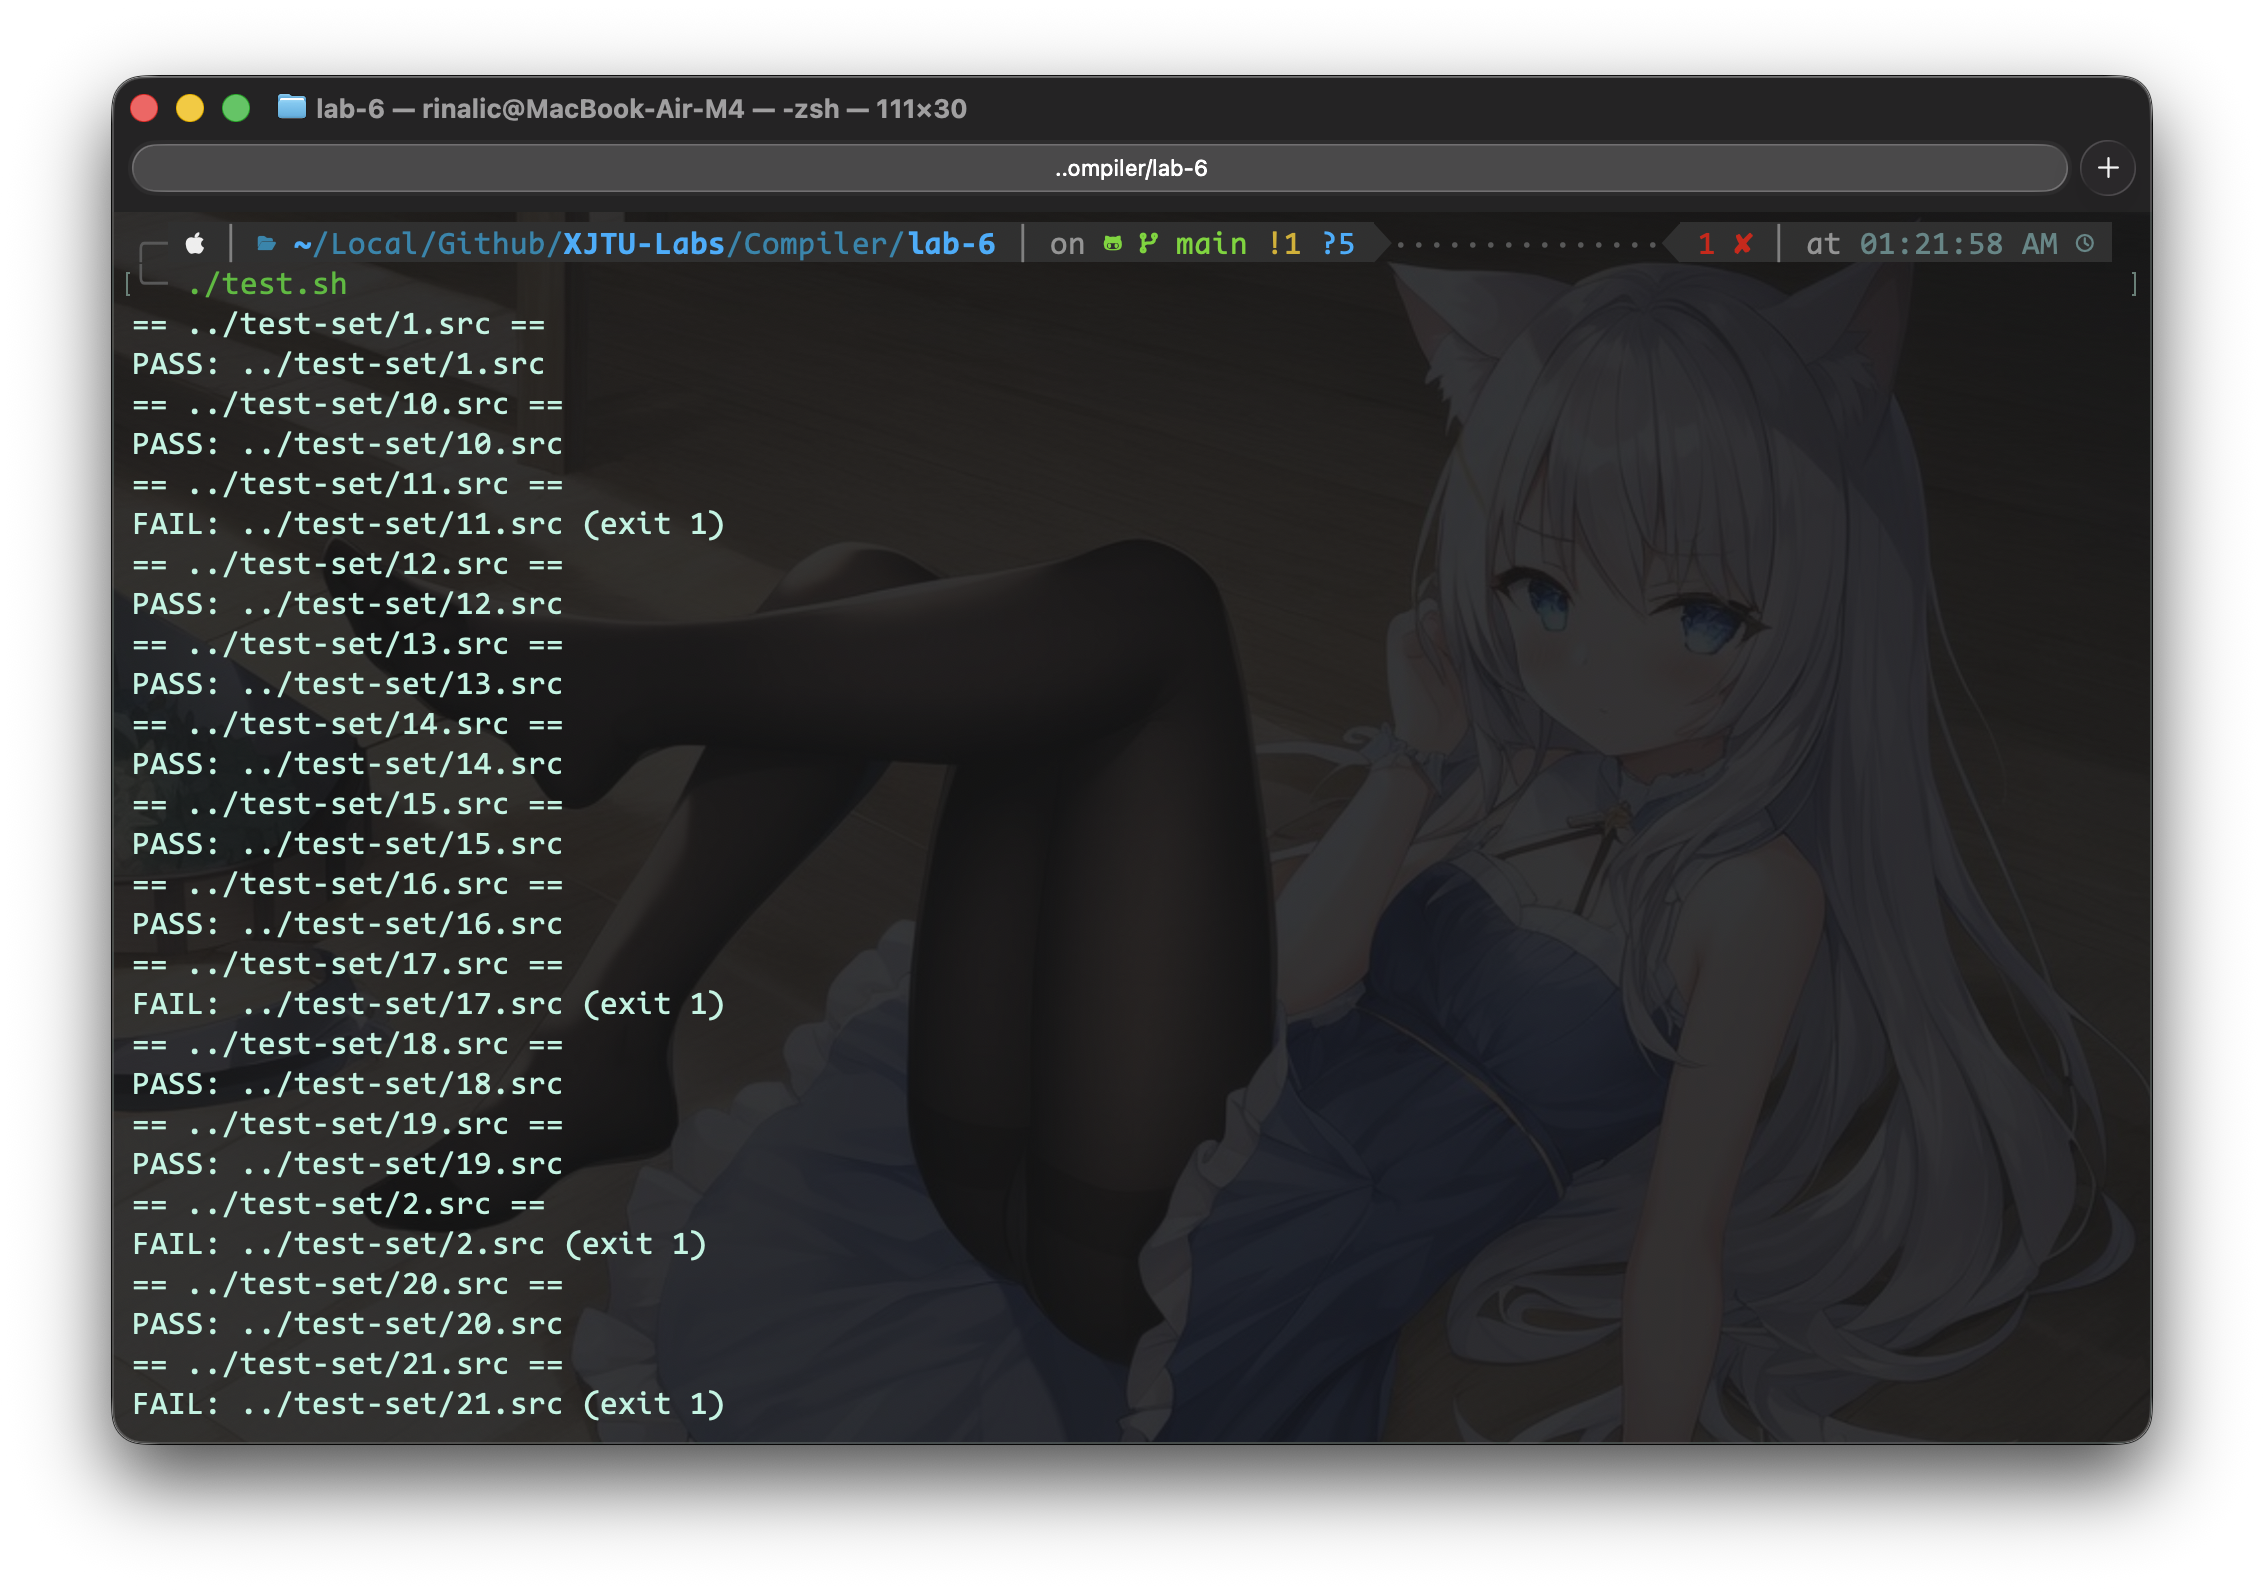
\includegraphics[width=0.9\textwidth]{images/run_test_script.png}
\caption{运行测试脚本并收集日志的终端截图}
\label{fig:run}
\end{figure}

说明：截图展示了在 `Compiler/lab-6` 目录下执行测试脚本 `test.sh` 并将标准输出、标准错误汇总到 `test-logs/all.out` 与 `test-logs/all.err` 的过程。截图中可以看到脚本对每个测试文件打印分隔符与 `STATUS`，便于后续人工或自动化检查。

\section{总结与体会}
本次实验实现了从词法分析、递归下降语法分析到中间四元组生成的完整前端流程，并加入了必要的语义检查以提高对错误输入的诊断能力。实现过程中的若干要点与体会如下：
\begin{itemize}
	\item 在实现递归下降解析器时，应避免在做前瞻检查时副作用修改词法器状态——一旦错误地前进了 token，后续解析会偏移并引入难以定位的错误。对此在实现中做了改进以保证 lookahead 安全。
	\item 为了避免解析器在遇到错误输入时进入无限循环，关键解析点（如 `parse\_primary`）在报告错误后会推进 token 至下一个可疑位置，从而保证解析器继续前进并发现更多错误。
	\item 测试驱动开发很重要：通过 `test-set` 中的样例，逐步调整语义规则（例如是否允许声明初始化）能让解析器行为与测试要求一致。
\end{itemize}

\section*{附录：主要源码}

\subsection*{A.1 测试脚本 \texttt{test.sh}}

\begin{lstlisting}
  out_dir=./test-logs
  mkdir -p "$out_dir"

  cc -std=c11 -O2 -Wall -Wextra -o icg main.c
  if [ $? -ne 0 ]; then
    echo "Build failed"
    exit 1
  fi

  out_file="$out_dir/all.out"
  err_file="$out_dir/all.err"
  tmp_err="$out_dir/.tmp.err"
  : > "$out_file"
  : > "$err_file"

  fail=0
  fail_list=""
  for f in ../test-set/*.src; do
    header="== $f =="
    echo "$header"
    echo "" >> "$out_file"
    echo "$header" >> "$out_file"
    echo "----------------------------------------" >> "$out_file"
    ./icg "$f" >> "$out_file" 2> "$tmp_err"
    exit_code=$?
    if [ $exit_code -ne 0 ]; then
      echo "" >> "$err_file"
      echo "$header" >> "$err_file"
      echo "----------------------------------------" >> "$err_file"
      cat "$tmp_err" >> "$err_file"
      echo "STATUS: FAIL (exit $exit_code)" >> "$err_file"
      echo "FAIL: $f (exit $exit_code)"
      fail=$((fail + 1))
      fail_list="$fail_list $f"
    else
      echo "STATUS: OK" >> "$out_file"
      echo "PASS: $f"
    fi
  done

  if [ $fail -ne 0 ]; then
    echo "FAIL: $fail case(s)"
    echo "FAILED:$fail_list"
    echo "See $out_file and $err_file for details"
    exit 1
  fi
  echo "ALL PASS"
  echo "See $out_file and $err_file for details"
\end{lstlisting}

\subsection*{A.2 运行与测试命令}
\begin{verbatim}
# 编译：
cc -std=c11 -O2 -Wall -Wextra -o icg main.c

# 逐个测试并收集日志（示例脚本已存在：test.sh）：
sh test.sh

# 手动对单个测试文件运行：
./icg ../test-set/1.src > out.txt 2> err.txt
\end{verbatim}

\subsection*{A.3 `main.c`}
\begin{lstlisting}
#include <ctype.h>
#include <stdio.h>
#include <stdlib.h>
#include <string.h>

#define MAX_SRC 65536
#define MAX_NAME 64
#define MAX_QUADS 4096
#define MAX_SYMBOLS 512
#define MAX_FUNCS 128
#define MAX_CALLS 512
#define MAX_ERRORS 256

typedef enum
{
	TOK_EOF = 0,
	TOK_ID,
	TOK_NUM,
	TOK_INT,
	TOK_FLOAT,
	TOK_VOID,
	TOK_IF,
	TOK_ELSE,
	TOK_WHILE,
	TOK_RETURN,
	TOK_PRINT,
	TOK_INPUT,
	TOK_LPA,
	TOK_RPA,
	TOK_LBR,
	TOK_RBR,
	TOK_LBK,
	TOK_RBK,
	TOK_COMMA,
	TOK_SEMI,
	TOK_ADD,
	TOK_SUB,
	TOK_MUL,
	TOK_DIV,
	TOK_ASSIGN,
	TOK_EQ,
	TOK_NE,
	TOK_LT,
	TOK_LE,
	TOK_GT,
	TOK_GE
} TokenType;

typedef struct
{
	TokenType type;
	char lexeme[MAX_NAME];
	int line;
	int col;
} Token;

typedef struct
{
	const char *src;
	size_t pos;
	int line;
	int col;
} Lexer;

typedef enum
{
	TYPE_UNKNOWN = 0,
	TYPE_INT,
	TYPE_FLOAT,
	TYPE_VOID
} ValueType;

typedef struct
{
	char name[MAX_NAME];
	ValueType type;
	int scope;
	int is_array;
	int array_size;
} Symbol;

typedef struct
{
	char name[MAX_NAME];
	ValueType ret_type;
} Function;

typedef struct
{
	char op[16];
	char arg1[MAX_NAME];
	char arg2[MAX_NAME];
	char res[MAX_NAME];
} Quad;

typedef struct
{
	char name[MAX_NAME];
	ValueType type;
	int is_lvalue;
} Expr;

static Lexer g_lex;
static Token g_cur;
static Quad g_quads[MAX_QUADS];
static int g_quad_count = 0;
static int g_temp_count = 0;
static Symbol g_symbols[MAX_SYMBOLS];
static int g_symbol_count = 0;
static Function g_funcs[MAX_FUNCS];
static int g_func_count = 0;
static char g_calls[MAX_CALLS][MAX_NAME];
static int g_call_count = 0;
static int g_scope_level = 0;
static ValueType g_func_ret = TYPE_VOID;
static char g_errors[MAX_ERRORS][MAX_NAME * 2];
static int g_error_count = 0;

static void
record_error (const char *msg)
{
	if (g_error_count >= MAX_ERRORS)
		{
			return;
		}
	strncpy (g_errors[g_error_count], msg, sizeof (g_errors[0]) - 1);
	g_errors[g_error_count][sizeof (g_errors[0]) - 1] = '\0';
	g_error_count++;
}

static void
lexer_init (const char *src)
{
	g_lex.src = src;
	g_lex.pos = 0;
	g_lex.line = 1;
	g_lex.col = 1;
}

static char
lexer_peek (void)
{
	return g_lex.src[g_lex.pos];
}

static char
lexer_next (void)
{
	char c = g_lex.src[g_lex.pos];
	if (c == '\0')
		{
			return c;
		}
	g_lex.pos++;
	if (c == '\n')
		{
			g_lex.line++;
			g_lex.col = 1;
		}
	else
		{
			g_lex.col++;
		}
	return c;
}

static void
skip_whitespace (void)
{
	while (1)
		{
			char c = lexer_peek ();
			if (isspace ((unsigned char)c))
				{
					lexer_next ();
					continue;
				}
			if (c == '/' && g_lex.src[g_lex.pos + 1] == '/')
				{
					while (c != '\0' && c != '\n')
						{
							c = lexer_next ();
						}
					continue;
				}
			if (c == '/' && g_lex.src[g_lex.pos + 1] == '*')
				{
					lexer_next ();
					lexer_next ();
					while (1)
						{
							c = lexer_peek ();
							if (c == '\0')
								{
									break;
								}
							if (c == '*' && g_lex.src[g_lex.pos + 1] == '/')
								{
									lexer_next ();
									lexer_next ();
									break;
								}
							lexer_next ();
						}
					continue;
				}
			break;
		}
}

static int
is_ident_start (char c)
{
	return isalpha ((unsigned char)c) || c == '_';
}

static int
is_ident_char (char c)
{
	return isalnum ((unsigned char)c) || c == '_';
}

static Token
make_token (TokenType type, const char *lexeme, int line, int col)
{
	Token t;
	t.type = type;
	strncpy (t.lexeme, lexeme, MAX_NAME - 1);
	t.lexeme[MAX_NAME - 1] = '\0';
	t.line = line;
	t.col = col;
	return t;
}

static Token
next_token (void)
{
	skip_whitespace ();
	int line = g_lex.line;
	int col = g_lex.col;
	char c = lexer_peek ();
	if (c == '\0')
		{
			return make_token (TOK_EOF, "", line, col);
		}

	if (is_ident_start (c))
		{
			char buf[MAX_NAME];
			int n = 0;
			while (is_ident_char (lexer_peek ()))
				{
					if (n < MAX_NAME - 1)
						{
							buf[n++] = lexer_next ();
						}
					else
						{
							lexer_next ();
						}
				}
			buf[n] = '\0';
			if (strcmp (buf, "int") == 0)
				{
					return make_token (TOK_INT, buf, line, col);
				}
			if (strcmp (buf, "float") == 0)
				{
					return make_token (TOK_FLOAT, buf, line, col);
				}
			if (strcmp (buf, "void") == 0)
				{
					return make_token (TOK_VOID, buf, line, col);
				}
			if (strcmp (buf, "if") == 0)
				{
					return make_token (TOK_IF, buf, line, col);
				}
			if (strcmp (buf, "else") == 0)
				{
					return make_token (TOK_ELSE, buf, line, col);
				}
			if (strcmp (buf, "while") == 0)
				{
					return make_token (TOK_WHILE, buf, line, col);
				}
			if (strcmp (buf, "return") == 0)
				{
					return make_token (TOK_RETURN, buf, line, col);
				}
			if (strcmp (buf, "print") == 0)
				{
					return make_token (TOK_PRINT, buf, line, col);
				}
			if (strcmp (buf, "input") == 0)
				{
					return make_token (TOK_INPUT, buf, line, col);
				}
			return make_token (TOK_ID, buf, line, col);
		}

	if (c == '.' && isdigit ((unsigned char)g_lex.src[g_lex.pos + 1]))
		{
			char buf[MAX_NAME];
			int n = 0;
			int has_dot = 0;
			while (isdigit ((unsigned char)lexer_peek ()) || lexer_peek () == '.')
				{
					if (lexer_peek () == '.')
						{
							if (has_dot)
								{
									break;
								}
							has_dot = 1;
						}
					if (n < MAX_NAME - 1)
						{
							buf[n++] = lexer_next ();
						}
					else
						{
							lexer_next ();
						}
				}
			buf[n] = '\0';
			return make_token (TOK_NUM, buf, line, col);
		}

	if (isdigit ((unsigned char)c))
		{
			char buf[MAX_NAME];
			int n = 0;
			int has_dot = 0;
			while (isdigit ((unsigned char)lexer_peek ()) || lexer_peek () == '.')
				{
					if (lexer_peek () == '.')
						{
							if (has_dot)
								{
									break;
								}
							has_dot = 1;
						}
					if (n < MAX_NAME - 1)
						{
							buf[n++] = lexer_next ();
						}
					else
						{
							lexer_next ();
						}
				}
			buf[n] = '\0';
			return make_token (TOK_NUM, buf, line, col);
		}

	lexer_next ();
	switch (c)
		{
		case '(':
			return make_token (TOK_LPA, "(", line, col);
		case ')':
			return make_token (TOK_RPA, ")", line, col);
		case '{':
			return make_token (TOK_LBR, "{", line, col);
		case '}':
			return make_token (TOK_RBR, "}", line, col);
		case '[':
			return make_token (TOK_LBK, "[", line, col);
		case ']':
			return make_token (TOK_RBK, "]", line, col);
		case ',':
			return make_token (TOK_COMMA, ",", line, col);
		case ';':
			return make_token (TOK_SEMI, ";", line, col);
		case '+':
			return make_token (TOK_ADD, "+", line, col);
		case '-':
			return make_token (TOK_SUB, "-", line, col);
		case '*':
			return make_token (TOK_MUL, "*", line, col);
		case '/':
			return make_token (TOK_DIV, "/", line, col);
		case '=':
			if (lexer_peek () == '=')
				{
					lexer_next ();
					return make_token (TOK_EQ, "==", line, col);
				}
			return make_token (TOK_ASSIGN, "=", line, col);
		case '!':
			if (lexer_peek () == '=')
				{
					lexer_next ();
					return make_token (TOK_NE, "!=", line, col);
				}
			break;
		case '<':
			if (lexer_peek () == '=')
				{
					lexer_next ();
					return make_token (TOK_LE, "<=", line, col);
				}
			return make_token (TOK_LT, "<", line, col);
		case '>':
			if (lexer_peek () == '=')
				{
					lexer_next ();
					return make_token (TOK_GE, ">=", line, col);
				}
			return make_token (TOK_GT, ">", line, col);
		default:
			break;
		}

	{
		char msg[MAX_NAME * 2];
		snprintf (msg, sizeof (msg), "Unexpected character '%c' at %d:%d", c, line,
							col);
		record_error (msg);
	}
	return make_token (TOK_EOF, "", line, col);
}

static void
advance_token (void)
{
	g_cur = next_token ();
}

static int
match (TokenType type)
{
	if (g_cur.type == type)
		{
			advance_token ();
			return 1;
		}
	return 0;
}

static void
expect (TokenType type, const char *msg)
{
	if (!match (type))
		{
			char err[MAX_NAME * 2];
			snprintf (err, sizeof (err), "%s at %d:%d", msg, g_cur.line, g_cur.col);
			record_error (err);
		}
}

static void
emit_quad (const char *op, const char *arg1, const char *arg2, const char *res)
{
	if (g_quad_count >= MAX_QUADS)
		{
			record_error ("Too many quadruples");
			return;
		}
	Quad *q = &g_quads[g_quad_count++];
	strncpy (q->op, op, sizeof (q->op) - 1);
	q->op[sizeof (q->op) - 1] = '\0';
	strncpy (q->arg1, arg1 ? arg1 : "", MAX_NAME - 1);
	q->arg1[MAX_NAME - 1] = '\0';
	strncpy (q->arg2, arg2 ? arg2 : "", MAX_NAME - 1);
	q->arg2[MAX_NAME - 1] = '\0';
	strncpy (q->res, res ? res : "", MAX_NAME - 1);
	q->res[MAX_NAME - 1] = '\0';
}

static int
current_quad_index (void)
{
	return g_quad_count + 1;
}

static void
patch_quad (int index, int target)
{
	if (index <= 0 || index > g_quad_count)
		{
			return;
		}
	char buf[MAX_NAME];
	snprintf (buf, sizeof (buf), "%d", target);
	strncpy (g_quads[index - 1].res, buf, MAX_NAME - 1);
	g_quads[index - 1].res[MAX_NAME - 1] = '\0';
}

static void
new_temp (char *out)
{
	snprintf (out, MAX_NAME, "T%d", ++g_temp_count);
}

static void
enter_scope (void)
{
	g_scope_level++;
}

static void
leave_scope (void)
{
	if (g_scope_level > 0)
		{
			g_scope_level--;
		}
}

static int
find_symbol (const char *name, ValueType *type)
{
	for (int i = g_symbol_count - 1; i >= 0; --i)
		{
			if (g_symbols[i].scope > g_scope_level)
				{
					continue;
				}
			if (strcmp (g_symbols[i].name, name) == 0)
				{
					if (type)
						{
							*type = g_symbols[i].type;
						}
					return 1;
				}
		}
	return 0;
}

static int
declare_symbol (const char *name, ValueType type, int is_array, int array_size)
{
	for (int i = 0; i < g_symbol_count; ++i)
		{
			if (g_symbols[i].scope == g_scope_level
					&& strcmp (g_symbols[i].name, name) == 0)
				{
					return 0;
				}
		}
	if (g_symbol_count >= MAX_SYMBOLS)
		{
			return 0;
		}
	Symbol *sym = &g_symbols[g_symbol_count++];
	strncpy (sym->name, name, MAX_NAME - 1);
	sym->name[MAX_NAME - 1] = '\0';
	sym->type = type;
	sym->scope = g_scope_level;
	sym->is_array = is_array;
	sym->array_size = array_size;
	return 1;
}

static int
find_function (const char *name, ValueType *ret_type)
{
	for (int i = 0; i < g_func_count; ++i)
		{
			if (strcmp (g_funcs[i].name, name) == 0)
				{
					if (ret_type)
						{
							*ret_type = g_funcs[i].ret_type;
						}
					return 1;
				}
		}
	return 0;
}

static int
declare_function (const char *name, ValueType ret_type)
{
	for (int i = 0; i < g_func_count; ++i)
		{
			if (strcmp (g_funcs[i].name, name) == 0)
				{
					return 0;
				}
		}
	if (g_func_count >= MAX_FUNCS)
		{
			return 0;
		}
	Function *fn = &g_funcs[g_func_count++];
	strncpy (fn->name, name, MAX_NAME - 1);
	fn->name[MAX_NAME - 1] = '\0';
	fn->ret_type = ret_type;
	return 1;
}

static void
record_call (const char *name)
{
	for (int i = 0; i < g_call_count; ++i)
		{
			if (strcmp (g_calls[i], name) == 0)
				{
					return;
				}
		}
	if (g_call_count >= MAX_CALLS)
		{
			return;
		}
	strncpy (g_calls[g_call_count], name, MAX_NAME - 1);
	g_calls[g_call_count][MAX_NAME - 1] = '\0';
	g_call_count++;
}

static void
check_undefined_calls (void)
{
	for (int i = 0; i < g_call_count; ++i)
		{
			if (!find_function (g_calls[i], NULL))
				{
					char msg[MAX_NAME * 2];
					snprintf (msg, sizeof (msg), "Undeclared function '%s'", g_calls[i]);
					record_error (msg);
				}
		}
}

static ValueType
type_merge (ValueType a, ValueType b)
{
	if (a == TYPE_FLOAT || b == TYPE_FLOAT)
		{
			return TYPE_FLOAT;
		}
	if (a == TYPE_INT && b == TYPE_INT)
		{
			return TYPE_INT;
		}
	return TYPE_UNKNOWN;
}

static Expr parse_expression (void);
static void parse_statement (void);
static void parse_block (void);

static Expr
make_expr (const char *name, ValueType type, int is_lvalue)
{
	Expr e;
	strncpy (e.name, name, MAX_NAME - 1);
	e.name[MAX_NAME - 1] = '\0';
	e.type = type;
	e.is_lvalue = is_lvalue;
	return e;
}

static Expr
parse_primary (void)
{
	if (g_cur.type == TOK_NUM)
		{
			Expr e = make_expr (g_cur.lexeme, TYPE_INT, 0);
			if (strchr (g_cur.lexeme, '.') != NULL)
				{
					e.type = TYPE_FLOAT;
				}
			advance_token ();
			return e;
		}

	if (g_cur.type == TOK_ID)
		{
			char name[MAX_NAME];
			strncpy (name, g_cur.lexeme, MAX_NAME - 1);
			name[MAX_NAME - 1] = '\0';
			advance_token ();

			if (match (TOK_LPA))
				{
					int arg_count = 0;
					if (g_cur.type != TOK_RPA)
						{
							while (1)
								{
									Expr arg = parse_expression ();
									emit_quad ("param", arg.name, "", "");
									arg_count++;
									if (match (TOK_COMMA))
										{
											if (g_cur.type == TOK_RPA)
												{
													record_error ("Trailing comma in call");
													break;
												}
											continue;
										}
									break;
								}
						}
					expect (TOK_RPA, "Missing ) in call");
					char tmp[MAX_NAME];
					new_temp (tmp);
					char argc_buf[MAX_NAME];
					snprintf (argc_buf, sizeof (argc_buf), "%d", arg_count);
					emit_quad ("call", name, argc_buf, tmp);
					ValueType ret_type = TYPE_UNKNOWN;
					if (!find_function (name, &ret_type))
						{
							record_call (name);
						}
					return make_expr (tmp, ret_type, 0);
				}

			char full[MAX_NAME];
			strncpy (full, name, MAX_NAME - 1);
			full[MAX_NAME - 1] = '\0';
			ValueType t = TYPE_UNKNOWN;
			if (!find_symbol (name, &t))
				{
					char msg[MAX_NAME * 2];
					snprintf (msg, sizeof (msg), "Undeclared identifier '%s'", name);
					record_error (msg);
				}

			while (match (TOK_LBK))
				{
					Expr idx = parse_expression ();
					expect (TOK_RBK, "Missing ]");
					char buf[MAX_NAME];
					snprintf (buf, sizeof (buf), "%s[%s]", full, idx.name);
					strncpy (full, buf, MAX_NAME - 1);
					full[MAX_NAME - 1] = '\0';
				}
			return make_expr (full, t, 1);
		}

	if (g_cur.type == TOK_INPUT)
		{
			advance_token ();
			expect (TOK_LPA, "Missing ( after input");
			expect (TOK_RPA, "Missing ) after input");
			char tmp[MAX_NAME];
			new_temp (tmp);
			emit_quad ("input", "", "", tmp);
			return make_expr (tmp, TYPE_INT, 0);
		}

	if (match (TOK_LPA))
		{
			Expr e = parse_expression ();
			expect (TOK_RPA, "Missing )");
			return e;
		}

	if (match (TOK_ADD))
		{
			Expr e = parse_primary ();
			return make_expr (e.name, e.type, 0);
		}

	if (match (TOK_SUB))
		{
			Expr e = parse_primary ();
			char tmp[MAX_NAME];
			new_temp (tmp);
			emit_quad ("neg", e.name, "", tmp);
			return make_expr (tmp, e.type, 0);
		}

	record_error ("Invalid expression");
	if (g_cur.type != TOK_EOF)
		{
			advance_token ();
		}
	return make_expr ("", TYPE_UNKNOWN, 0);
}

static Expr
parse_term (void)
{
	Expr left = parse_primary ();
	while (g_cur.type == TOK_MUL || g_cur.type == TOK_DIV)
		{
			TokenType op = g_cur.type;
			advance_token ();
			Expr right = parse_primary ();
			char tmp[MAX_NAME];
			new_temp (tmp);
			emit_quad (op == TOK_MUL ? "*" : "/", left.name, right.name, tmp);
			left = make_expr (tmp, type_merge (left.type, right.type), 0);
		}
	return left;
}

static Expr
parse_additive (void)
{
	Expr left = parse_term ();
	while (g_cur.type == TOK_ADD || g_cur.type == TOK_SUB)
		{
			TokenType op = g_cur.type;
			advance_token ();
			Expr right = parse_term ();
			char tmp[MAX_NAME];
			new_temp (tmp);
			emit_quad (op == TOK_ADD ? "+" : "-", left.name, right.name, tmp);
			left = make_expr (tmp, type_merge (left.type, right.type), 0);
		}
	return left;
}

static Expr
parse_assignment_expr (void)
{
	Expr left = parse_additive ();
	if (g_cur.type == TOK_ASSIGN)
		{
			if (!left.is_lvalue)
				{
					record_error ("Left side of assignment is not assignable");
				}
			advance_token ();
			Expr right = parse_assignment_expr ();
			emit_quad ("=", right.name, "", left.name);
			left.is_lvalue = 0;
			left.type = right.type;
		}
	return left;
}

static Expr
parse_expression (void)
{
	return parse_assignment_expr ();
}

static void
parse_condition (char *op_out, Expr *left_out, Expr *right_out)
{
	Expr left = parse_expression ();
	if (g_cur.type == TOK_LT || g_cur.type == TOK_LE || g_cur.type == TOK_GT
			|| g_cur.type == TOK_GE || g_cur.type == TOK_EQ || g_cur.type == TOK_NE)
		{
			TokenType op = g_cur.type;
			advance_token ();
			Expr right = parse_expression ();
			const char *op_str = "";
			switch (op)
				{
				case TOK_LT:
					op_str = "j<";
					break;
				case TOK_LE:
					op_str = "j<=";
					break;
				case TOK_GT:
					op_str = "j>";
					break;
				case TOK_GE:
					op_str = "j>=";
					break;
				case TOK_EQ:
					op_str = "j==";
					break;
				case TOK_NE:
					op_str = "j!=";
					break;
				default:
					break;
				}
			strncpy (op_out, op_str, 8);
			*left_out = left;
			*right_out = right;
			return;
		}

	strncpy (op_out, "j!=", 8);
	*left_out = left;
	*right_out = make_expr ("0", TYPE_INT, 0);
}

static void
parse_decl (ValueType type)
{
	while (1)
		{
			if (g_cur.type != TOK_ID)
				{
					record_error ("Expected identifier in declaration");
					return;
				}
			char name[MAX_NAME];
			strncpy (name, g_cur.lexeme, MAX_NAME - 1);
			name[MAX_NAME - 1] = '\0';
			advance_token ();

			int is_array = 0;
			int array_size = 0;
			if (match (TOK_LBK))
				{
					if (g_cur.type == TOK_NUM)
						{
							array_size = atoi (g_cur.lexeme);
							advance_token ();
						}
					else
						{
							record_error ("Array size must be number");
						}
					expect (TOK_RBK, "Missing ] in array");
					is_array = 1;
				}

			if (!declare_symbol (name, type, is_array, array_size))
				{
					char msg[MAX_NAME * 2];
					snprintf (msg, sizeof (msg), "Duplicate declaration of '%s'", name);
					record_error (msg);
				}

			if (match (TOK_ASSIGN))
				{
					record_error ("Initialization in declaration is not allowed");
					(void)parse_expression ();
				}

			if (match (TOK_COMMA))
				{
					continue;
				}
			break;
		}
}

static void
parse_if (void)
{
	expect (TOK_IF, "Expected if");
	expect (TOK_LPA, "Missing ( after if");
	char op[8] = "";
	Expr left, right;
	parse_condition (op, &left, &right);
	expect (TOK_RPA, "Missing ) after if condition");

	int true_jump = current_quad_index ();
	emit_quad (op, left.name, right.name, "");
	int false_jump = current_quad_index ();
	emit_quad ("j", "", "", "");

	parse_statement ();
	if (g_cur.type == TOK_ELSE)
		{
			int end_jump = current_quad_index ();
			emit_quad ("j", "", "", "");
			patch_quad (true_jump, true_jump + 2);
			patch_quad (false_jump, current_quad_index ());
			advance_token ();
			parse_statement ();
			patch_quad (end_jump, current_quad_index ());
		}
	else
		{
			patch_quad (true_jump, true_jump + 2);
			patch_quad (false_jump, current_quad_index ());
		}
}

static void
parse_while (void)
{
	expect (TOK_WHILE, "Expected while");
	int loop_start = current_quad_index ();
	expect (TOK_LPA, "Missing ( after while");
	char op[8] = "";
	Expr left, right;
	parse_condition (op, &left, &right);
	expect (TOK_RPA, "Missing ) after while condition");

	int true_jump = current_quad_index ();
	emit_quad (op, left.name, right.name, "");
	int false_jump = current_quad_index ();
	emit_quad ("j", "", "", "");

	parse_statement ();
	emit_quad ("j", "", "", "");
	patch_quad (g_quad_count, loop_start);
	patch_quad (true_jump, true_jump + 2);
	patch_quad (false_jump, current_quad_index ());
}

static void
parse_return (void)
{
	expect (TOK_RETURN, "Expected return");
	if (g_cur.type != TOK_SEMI && g_cur.type != TOK_RBR)
		{
			Expr e = parse_expression ();
			if (g_func_ret == TYPE_VOID)
				{
					record_error ("Void function should not return a value");
				}
			else if (g_func_ret == TYPE_INT && e.type == TYPE_FLOAT)
				{
					record_error ("Return type mismatch (float to int)");
				}
			emit_quad ("ret", e.name, "", "");
		}
	else
		{
			if (g_func_ret != TYPE_VOID)
				{
					record_error ("Non-void function should return a value");
				}
			emit_quad ("ret", "", "", "");
		}
	match (TOK_SEMI);
}

static void
parse_print (void)
{
	expect (TOK_PRINT, "Expected print");
	if (match (TOK_LPA))
		{
			Expr e = parse_expression ();
			expect (TOK_RPA, "Missing ) after print");
			emit_quad ("print", e.name, "", "");
		}
	else
		{
			Expr e = parse_expression ();
			emit_quad ("print", e.name, "", "");
		}
	match (TOK_SEMI);
}

static void
parse_statement (void)
{
	if (g_cur.type == TOK_LBR)
		{
			parse_block ();
			return;
		}
	if (g_cur.type == TOK_IF)
		{
			parse_if ();
			return;
		}
	if (g_cur.type == TOK_WHILE)
		{
			parse_while ();
			return;
		}
	if (g_cur.type == TOK_RETURN)
		{
			parse_return ();
			return;
		}
	if (g_cur.type == TOK_PRINT)
		{
			parse_print ();
			return;
		}
	if (g_cur.type == TOK_INT || g_cur.type == TOK_FLOAT)
		{
			ValueType t = g_cur.type == TOK_INT ? TYPE_INT : TYPE_FLOAT;
			advance_token ();
			parse_decl (t);
			match (TOK_SEMI);
			return;
		}
	Expr e = parse_expression ();
	(void)e;
	match (TOK_SEMI);
}

static void
parse_block (void)
{
	expect (TOK_LBR, "Missing {");
	enter_scope ();
	while (g_cur.type != TOK_RBR && g_cur.type != TOK_EOF)
		{
			parse_statement ();
		}
	expect (TOK_RBR, "Missing }");
	leave_scope ();
	match (TOK_SEMI);
}

static ValueType
parse_type_spec (void)
{
	if (g_cur.type == TOK_INT)
		{
			advance_token ();
			return TYPE_INT;
		}
	if (g_cur.type == TOK_FLOAT)
		{
			advance_token ();
			return TYPE_FLOAT;
		}
	if (g_cur.type == TOK_VOID)
		{
			advance_token ();
			return TYPE_VOID;
		}
	record_error ("Expected type");
	return TYPE_UNKNOWN;
}

static void
parse_params (void)
{
	if (g_cur.type == TOK_RPA)
		{
			return;
		}
	while (1)
		{
			ValueType t = parse_type_spec ();
			if (g_cur.type != TOK_ID)
				{
					record_error ("Expected parameter name");
					return;
				}
			char name[MAX_NAME];
			strncpy (name, g_cur.lexeme, MAX_NAME - 1);
			name[MAX_NAME - 1] = '\0';
			advance_token ();
			if (!declare_symbol (name, t, 0, 0))
				{
					char msg[MAX_NAME * 2];
					snprintf (msg, sizeof (msg), "Duplicate declaration of '%s'", name);
					record_error (msg);
				}
			if (match (TOK_COMMA))
				{
					if (g_cur.type == TOK_RPA)
						{
							record_error ("Trailing comma in params");
							return;
						}
					continue;
				}
			break;
		}
}

static void
parse_function (void)
{
	ValueType ret_type = parse_type_spec ();
	if (g_cur.type != TOK_ID)
		{
			record_error ("Expected function name");
			return;
		}
	char name[MAX_NAME];
	strncpy (name, g_cur.lexeme, MAX_NAME - 1);
	name[MAX_NAME - 1] = '\0';
	advance_token ();

	if (!declare_function (name, ret_type))
		{
			char msg[MAX_NAME * 2];
			snprintf (msg, sizeof (msg), "Duplicate function '%s'", name);
			record_error (msg);
		}

	expect (TOK_LPA, "Missing ( in function");
	enter_scope ();
	g_func_ret = ret_type;
	parse_params ();
	expect (TOK_RPA, "Missing ) in function");
	parse_block ();
	leave_scope ();
	(void)name;
}

static void
parse_toplevel (void)
{
	while (g_cur.type != TOK_EOF)
		{
			if (g_cur.type == TOK_INT || g_cur.type == TOK_FLOAT
					|| g_cur.type == TOK_VOID)
				{
					parse_function ();
				}
			else
				{
					parse_statement ();
				}
		}
}

static const char *
print_arg (const char *s)
{
	return s[0] ? s : " ";
}

static void
print_quads (void)
{
	for (int i = 0; i < g_quad_count; ++i)
		{
			Quad *q = &g_quads[i];
			printf ("%d. (%s, %s, %s, %s)\n", i + 1, print_arg (q->op),
							print_arg (q->arg1), print_arg (q->arg2), print_arg (q->res));
		}
}

int
main (int argc, char **argv)
{
	const char *path = NULL;
	if (argc >= 2)
		{
			path = argv[1];
		}
	FILE *fp = stdin;
	if (path)
		{
			fp = fopen (path, "r");
			if (!fp)
				{
					fprintf (stderr, "Cannot open input file: %s\n", path);
					return 1;
				}
		}

	char *src = calloc (1, MAX_SRC);
	if (!src)
		{
			fprintf (stderr, "Out of memory\n");
			return 1;
		}
	size_t nread = fread (src, 1, MAX_SRC - 1, fp);
	src[nread] = '\0';
	if (fp != stdin)
		{
			fclose (fp);
		}

	lexer_init (src);
	advance_token ();
	parse_toplevel ();
	check_undefined_calls ();

	if (g_error_count > 0)
		{
			for (int i = 0; i < g_error_count; ++i)
				{
					fprintf (stderr, "Error: %s\n", g_errors[i]);
				}
			free (src);
			return 1;
		}

	print_quads ();
	free (src);
	return 0;
}
\end{lstlisting}

\end{document}

